%%%%%%%%%%%%%%%%%%%%%%%%%%%%%%%%%%%%%%%%%
% Science Publications
% LaTeX Template
% Version 1 (1/5/2018)
%
% Original author:
% Ali Asfour (ali.f.asfour@gmail.com)
%
%%%%%%%%%%%%%%%%%%%%%%%%%%%%%%%%%%%%%%%%%

%----------------------------------------------------------------------------------------
%	PACKAGES AND OTHER DOCUMENT CONFIGURATIONS
%----------------------------------------------------------------------------------------
\documentclass[fleqn,10pt]{thescipub} % Document font size and equations flushed left
%\usepackage{fontspec}
%\fontspec[WordSpace=0.5]{Times New Roman}
\usepackage{natbib} 
\usepackage[english]{babel} % Specify a different language here - english by default
%----------------------------------------------------------------------------------------
%	Justification align and remove hyphenation
%----------------------------------------------------------------------------------------
\tolerance=1
\emergencystretch=\maxdimen
\hyphenpenalty=10000
\hbadness=10000
\usepackage{indentfirst}
\setlength{\parindent}{0.5cm}
%----------------------------------------------------------------------------------------
%	COLUMNS
%----------------------------------------------------------------------------------------

\setlength{\columnsep}{0.76cm} % Distance between the two columns of text
\setlength{\fboxrule}{0.75pt} % Width of the border around the abstract

%----------------------------------------------------------------------------------------
%	COLORS
%----------------------------------------------------------------------------------------

\definecolor{color3}{RGB}{25,72,126} % Color of the boxes behind the abstract and headings

%----------------------------------------------------------------------------------------
%	HYPERLINKS
%----------------------------------------------------------------------------------------

\usepackage{hyperref} % Required for hyperlinks
\hypersetup{hidelinks,colorlinks,breaklinks=true,urlcolor=black,citecolor=black,linkcolor=black,bookmarksopen=false,pdftitle={Title},pdfauthor={Author}}

%----------------------------------------------------------------------------------------
%	ARTICLE INFORMATION
%----------------------------------------------------------------------------------------
\JournalInfo{Journal Name} % Journal information

\PaperTitle{Paper Title} 
\Authors{First Author\textsuperscript{1}, Second Author\textsuperscript{2}, Third Author\textsuperscript{3}, Fourth Author\textsuperscript{4}} % Authors
\affiliation{\textsuperscript{1}\textit{Department Name, Name of Organization, City, Country;}} % Author affiliation
\affiliation{\textsuperscript{2}\textit{Department Name, Name of Organization, City, Country;}} % Author affiliation
\affiliation{\textsuperscript{3}\textit{Department Name, Name of Organization, City, Country;}} % Author affiliation
\affiliation{\textsuperscript{4}\textit{Department Name, Name of Organization, City, Country;}} % Author affiliation


\Keywords{Article Keywords List} % Keywords - if you don't want any simply remove all the text between the curly brackets
\newcommand{\keywordname}{Keywords} % Defines the keywords heading name

%----------------------------------------------------------------------------------------
%	ABSTRACT
%----------------------------------------------------------------------------------------

\Abstract{This electronic document is a “live” template. The various components of your paper [title, text, tables, figures and references] are already defined on the style sheet, as illustrated by the portions given in this document.}

%----------------------------------------------------------------------------------------

\begin{document}
\captionsetup[figure]{labelfont={bf},name={Fig.},labelsep=period}
\captionsetup[table]{labelfont={bf},name={Table},labelsep=period}
\flushbottom % Makes all text pages the same height

\maketitle % Print the title and abstract box

%----------------------------------------------------------------------------------------
%	ARTICLE CONTENTS
%----------------------------------------------------------------------------------------

\section*{Introduction} This template, created for LaTex, provides authors with most of the formatting specifications given in the instructions to authors and needed for preparing electronic versions of their papers. All standard paper components have been specified for three reasons: (a) ease of use when formatting individual papers, (b) automatic compliance to electronic requirements that facilitate the production of electronic products, and (c) conformity of style throughout a journal paper. Margins, column widths, line spacing, and type styles are built-in.  Examples of the type styles are provided throughout this document and are identified in type, within parentheses.

\section{Ease of Use}
\subsection{Selecting a Template}
This template has been tailored for output on the custom paper size (8.26 cm x 11.22 cm). The margins are set as follows: top = 0.98 mm, bottom = 1.18 mm, right = 0.79 mm, left = 0.79 mm, space between column = 0.3 mm. The paragraphs must be indented. All paragraphs must be left justified and right justified.

\subsection{Maintaining the Integrity of the Specifications} 
The template is used to format your paper and style the text. All margins, column widths, line spaces, and text fonts are prescribed; please do not alter them. Your paper is one part of the entire proceedings, not an independent document. Please do not revise any of the current designations.

Text font. The entire document should be in times New Roman font size 10. Paper title must be Left size, bold, regular font size 18 and the first letter of each word capitalized. Author names must be regular font size 10, bold. Author affiliation must be regular font size 9. Email addresses font size 9. Level 1 main headings must be Left size, bold, regular font size 12 and first word capitalized. Level 2 Sub headings must be left-justified, bold, italic, font size 11 and the first letter of each word capitalized.

\section{Prepare Your Paper Before Styling}
Before you begin to format your paper, first write and save the content as a separate text file. Keep your text and graphic files separate until after the text has been formatted and styled. Do not use hard tabs, and limit use of hard returns to only one return at the end of a paragraph. Do not add any kind of pagination anywhere in the paper. Do not number text heads-the template will do that for you.

\subsection{Abbreviations and Acronyms} 
Define abbreviations and acronyms the first time they are used in the text, even after they have been defined in the abstract. Do not use abbreviations in the title or headings unless they are unavoidable.

\subsection{Units} 
Use SI as primary units. English units may be used as secondary units (in parentheses). Use a zero before decimal points: “0.25”, not “.25”. Use “cm3”, not “cc”.

\subsection{Equations} 
The equations are an exception to the prescribed specifications of this template. You will need to determine whether or not your equation should be typed using either the Times New Roman or the Symbol font, Equations font size should be 9 and italic (please no other font). Equations should be edited by Math type, not in text or graphic versions. Number equations consecutively. Equation numbers, within parentheses, are to position flush right, as in (1), using a right tab stop.
\linebreak

Where:
\begin{itemize}
\item MC is the moisture content (\%)
\item M1 is the initial weight of the wet sample (g)
\item M2 is the weight of the dried sample (g)
\end{itemize}

Be sure that the symbols in your equation have been defined immediately following the equation. Use “Eq. 1”, not “Eq. (1)” or “Equation (1)”, and at the beginning of a sentence.

\section{Using the Template}
After the text edit has been completed, the paper is ready for the template. Duplicate the template file by using the Save As command. In this newly created file, highlight all of the contents and import your prepared text file. You are now ready to style your paper.

\subsection{Authors and Affiliations} 
The template is designed so that author affiliations are not repeated each time for multiple authors of the same affiliation. Please keep your affiliations as succinct as possible (do NOT post your job titles, positions, academic degrees, zip codes, names of building, street, district, province, state, etc.). This template was designed for two affiliations. You can adjust the template for authors with one affiliation or more than two affiliations.


\subsection{Identify the Headings} 
Sometimes mobile app Headings are organizational devices that guide the reader through your paper. There are two types: component headings and text heads. Component headings identify the different components of your paper and are not subordinate to each other. Examples include Introduction, Acknowledgments and References. Text heading organize the topics on a relational, hierarchical basis. If there are two or more sub-topics, the next level head should be used if there are not at least two sub-topics, then no subheads should be introduced.

\begin{figure*}[ht]\centering % Using \begin{figure*} makes the figure take up the entire width of the page
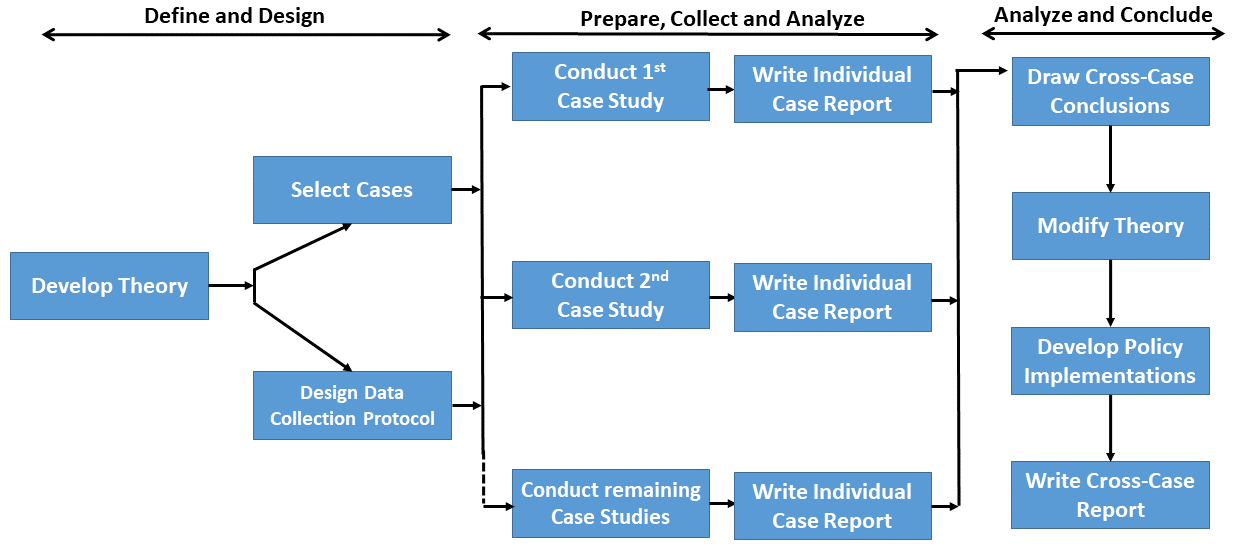
\includegraphics[width=\linewidth]{Multiple_case-study_design}
\caption{Multiple Case Study Design \citep{yin2013case}}
\label{Fig.Multiple_case-study_design}
\end{figure*}

\begin{table*}[!hbt]
\caption{Demographics of four cases}
\centering
\begin{tabular}{ p{3cm}  p{3cm} p{3cm} p{3cm} p{3cm} }
\toprule
Case ID &   C1	&	C2	&	C3	&	C4 \\
\midrule
Business type & Software house & Software house & Software house & Software house \\
Software house & National & International & International & National\\
Dev. Method & Scrum Agile & Kanban Agile & Scrum Agile & Scrum Agile \\
Mobile apps types & Games apps, Taxi apps & Business apps & Social apps, business apps & Hotel apps, travel apps\\
Single user/ Enterprise apps & Single user& Enterprise & Enterprise&Single user \\
Team size& 2 teams, each 5 members & 4 teams, each has 4 members & 5 teams, each has 5 members & 2 teams, each has 4 members\\
\bottomrule
\end{tabular}
\label{table:demographics_info}
\end{table*}

\subsection{Figures and Tables} 
Place figures and tables at the top or bottom of columns. Avoid placing them in the middle of columns. Large figures and tables may span across both columns. Figure captions should be below the figures; table heads should appear above the tables. Insert figures and tables after they are cited in the text. Use “Fig. 1” and “Table 1” even at the beginning of a sentence.

Use Times New Roman font size 9 for Figure and Table labels. Use words rather than symbols or abbreviations when writing Figure axis labels to avoid confusing the reader. If include-ing units in the label, present them within parentheses. Label axes only with units just “A/m”. Do not label axes with a ratio of quantities and units. Graphs may be full color. Use only SOLID FILL COLORS which contrast well both on screen and hardcopy as shown in Fig. 1. When using photographs make sure the resolution is adequate to reveal important details as shown in Fig. 2.

\section{Conclusion}
The main conclusions of the experimental work should be presented. The contribution of the work to the scientific community and its economic implications should be emphasized.

\section{Acknowledgement}
Use same font size for the content of acknowledgements section.

\section{Funding Information}
The authors should acknowledge the funders of this manuscript and provide all necessary funding information.

\section{Author’s Contributions}
This section should state the contributions made by each author in the preparation, development and publication of this manuscript.

\section{Ethics}
Authors should address any ethical issues that may arise after the publication of this manuscript.


\section{References}
Use the author/date system of references. In the text refer to the authors’ name (without initials) and year of publication. All publications cited in the text should be presented in a list of references following the text of the manuscript.

\begin{enumerate}
\item \subsection{Examples for a single author}
Peterson (1993) has shown that...This is in agreement with the results obtained by several authors (Kramer, 1994; Smith, 1995; Brown, 1999)
\item \subsection{Examples for two authors}
Smith and White (1999) reported that....This was later found to be incorrect (Amir and Ahmed, 2000).

\item \subsection{Examples for three or more authors}
Moore et al. (1990) stated that...Similar results were reported recently (Smith et al., 2003).
\end{enumerate}

The list of references should include only those cited in the manuscript and arranged alphabetically by authors’ names. Titles of journals should be given in full. ‘In press' can only be used to cite manuscripts actually accepted for publication in a journal. Citations such as ‘manuscript in preparation' or ‘manuscript submitted' are not permitted. Authors must provide Digital Object Identifier (DOI) number for all references. If there is no DOI for any reference, author may provide its URL/direct accessible web link for verification purpose. References without DOI or internet link are not acceptable.  The following format should be adhered to.

\begin{enumerate}
\item \subsection{Journal Papers}
Calik, P., P. Yilgora, P. Ayhanb and A.S. Demir. 2004. Oxygen transfer effects on recombinant benzaldehydelyase production. Chemical Engineering and Science, 59 (22-23): 5075-5083. DOI:10.1016/j.ces.2004.07.070.
\item \subsection{Text Book}
Navabi, Z., 1998. Analysis and Modeling of Digital Systems.2nd Ed. McGraw Hill, New York. ISBN: 0070464790, pp: 632.
\item \subsection{Book Chapter} Katz, R.H., 1986. Computer-Aided Design Databases. In: New Directions for Database Systems, Ariav, G. and J. Clifford, (Eds.), Intellect Books, Norwood, NJ, pp: 110-123. ISBN: 0893913448.
\item \subsection{Conference Proceedings} Magott, J. and K. Skudlarski, 1989. Combining Generalized Stochastic Petri Nets and PERT Networks For The Performance Evaluation Of Concurrent Processes. Proceedings of the 3rd International Workshop on Petri Nets and Performance Models, Dec. 11-13, IEEE Xplore Press, Japan, pp: 249-256. DOI: 10.1109/PNPM.1989.68558.
\item \subsection{Government Publications} United Nations, 2001. Indicators of Sustainable Development: Guidelines and Methodologies. United Nations Press, New York, USA.
\item \subsection{Online Publications} Lal, R., 1995. Sustainable Management of Soil Resources in the Humid Tropics. United Nations University Press, Tokyo, Japan. {URL} (Accessed on March 17, 2011)
\item \subsection{Generic Website}
UNEP, 2002.Cleaner Production Assessment in Industries.Production and Consumption Branch. United Nations Environment Program. {URL} (Accessed on February 13, 2011)
\item \subsection{Theses}
Alkoaik, F., 2005. Fate of plant pathogens and pesticides during composting of greenhouse tomato plant residues. Unpublished dissertation in partial fulfillment of the requirements for the degree of Doctor of Philosophy, Dalhousie University, Halifax, Nova Scotia, Canada
\end{enumerate}

%-------------------------------------------------------------------------
%	REFERENCE LIST
%----------------------------------------------------------------------------------------
\phantomsection
\setlength{\bibsep}{0.5pt} % remove spaces between references
\bibliographystyle{apalike} 
\bibliography{references}
%----------------------------------------------------------------------------------------

\end{document}